

% ─────────────────────────────────────────────────────────────────────────────
\section{Flowgraph description}
\label{sec:overview}
% ─────────────────────────────────────────────────────────────────────────────

\subsection*{Flowgraph overview}

Figure~\ref{fig:grc_overview} shows the full GRC canvas. The flowgraph is split into multiple zones that are highlighted : the simulation source, the SDR testbed, the parameter zones, receiver chain and the packet statistics.

\begin{figure}
  \centering
  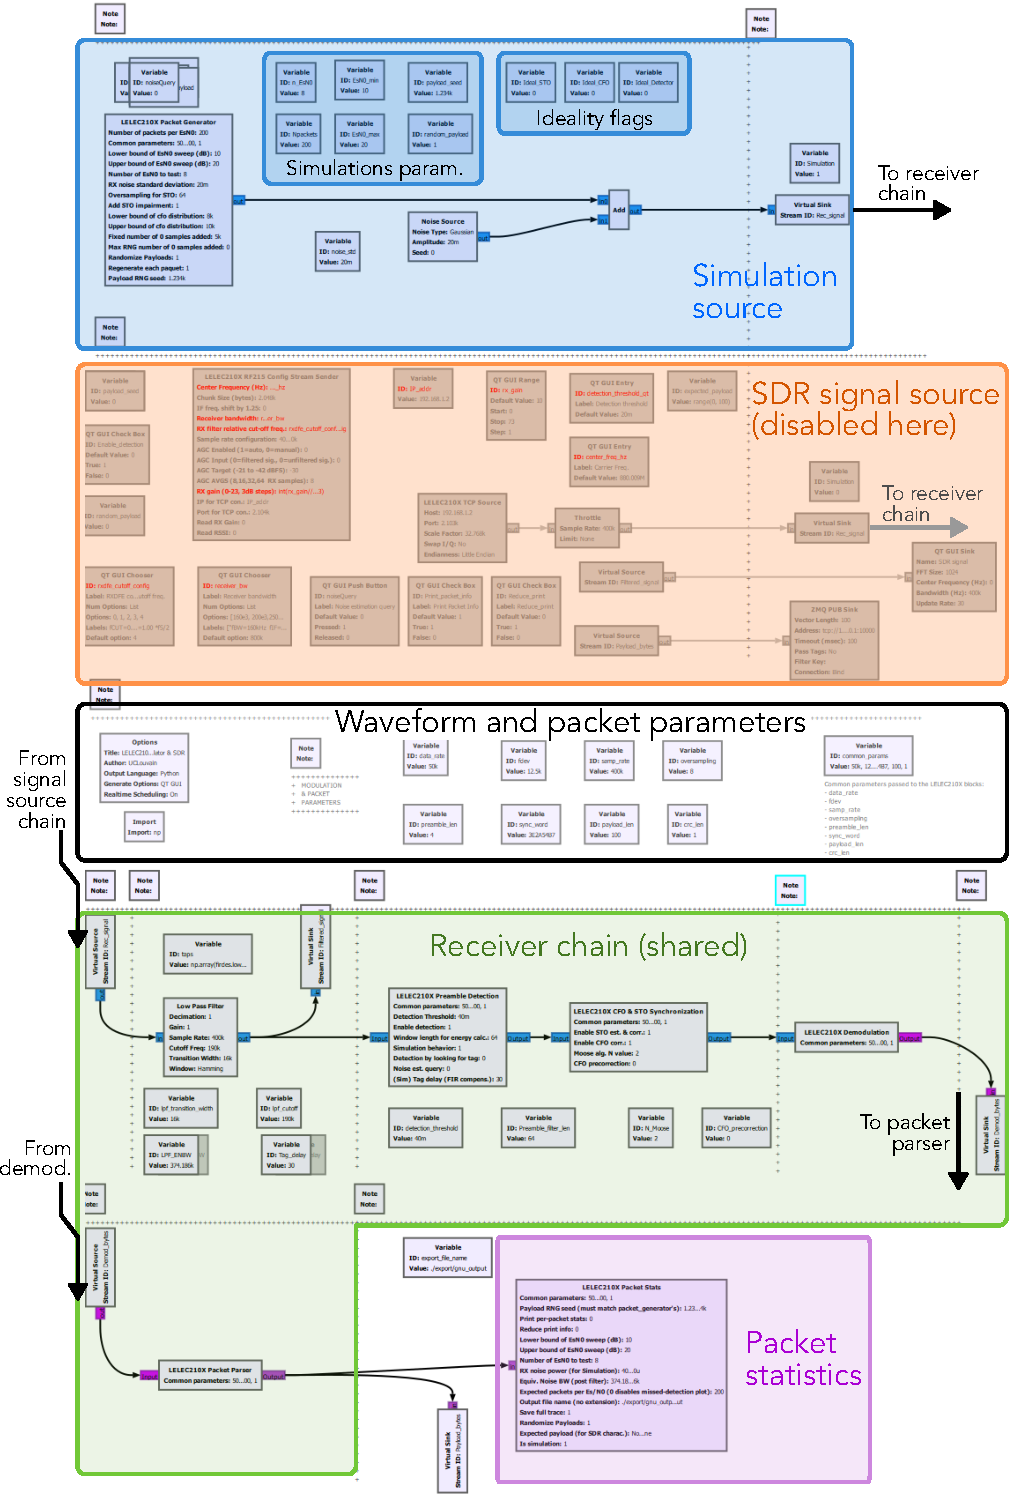
\includegraphics[width=\linewidth]{./figures/Flowgraph_edited.pdf}
  \caption{Full view of the \texttt{Project\_210X.grc} canvas with annotation for the different parts.}
  \label{fig:grc_overview}
\end{figure}

\subsection*{Step-by-step description}

\begin{enumerate}
  \item \textbf{Signal source.}
    In simulation mode, \texttt{packet\_generator} produces a continuous CP-FSK stream with configurable noise, CFO, and STO applied for each $\sfrac{\epsilon}{N_0}$ point.
    In SDR mode, \texttt{tcp\_source} receives 16-bit IQ samples from the
    AT86RF215 board over TCP and re-scales them to floating-point; the companion     block \texttt{rf215\_cfg\_stream\_sender} programs the radio's registers  (carrier frequency, IF bandwidth, gain) before streaming starts.
    Both sources feed the \texttt{Rec\_signal} virtual wire.

  \item \textbf{Low-pass FIR filter.}
    A symmetric  FIR with a default 190 kHz passband and 32 kHz
    transition band removes out-of-band noise and interference.
    Its group delay is exactly $\lfloor N/2 \rfloor$ samples, where $N$ is the tap count.
    The variable \texttt{Tag\_delay}~$= \lfloor \mathtt{len(taps)} / 2 \rfloor$ is passed to the downstream blocks so that event tags (preamble position, etc.) are time-aligned with the filtered output.

  \item \textbf{Preamble detection.}
    The detector evaluates the signal energy over a window of length $L =
    \mathtt{Preamble\_filter\_len}$, detects the energy signature of the
    alternating-preamble. On detection the block:
    \begin{itemize}
      \item emits the detected packet frame on its output;
      \item attaches the \texttt{detection\_latency} tag (number of samples by which detection lags the ideal packet start);
      \item attaches the \texttt{est\_noise\_power} tag (noise power measured during idle periods, if available);
      \item in simulation mode, forwards all generator tags (ground-truth CFO, STO, $\sfrac{\epsilon}{N_0}$, payload ID).
    \end{itemize}

  \item \textbf{Synchronisation.}
    The \textbf{Moose} algorithm estimates CFO from two consecutive blocks of $N_{\mathrm{Moose}}$ preamble symbols, then corrects every output sample.
    STO is estimated by maximising the sharpness of phase transitions across the
    preamble and used to align the symbol grid.
    Three tags are added: \texttt{est\_cfo}, \texttt{est\_sto},
    \texttt{est\_sig\_pow}.

  \item \textbf{Non-coherent FSK demodulation.}
    Each symbol (OSR complex samples) is correlated against the two reference  tones at $\pm f_{\mathrm{dev}}$ and the bit is decided by the stronger
    correlation. The result is a stream of raw bytes on the \textbf{Demod\_bytes}
    virtual wire.

  \item \textbf{Packet parsing.}
    The byte stream is correlated against the sync word to locate the frame
    boundary. The payload is extracted and CRC-checked; the block emits the
    payload vector tagged with \texttt{crc\_ok}, \texttt{payload\_start}, and     (in simulation) \texttt{payload\_id}.

  \item \textbf{Packet statistics (sink).}
    Every tag on the arriving payload vector is collected into a per-packet
    record. When the flowgraph stops the block saves performance curves (BER, PER, miss-detection rate, CFO RMSE, STO RMSE) grouped by $\sfrac{\epsilon}{N_0}$ and exports  CSV files and PNG plots. A CFO histogram is always produced.
\end{enumerate}



% ─────────────────────────────────────────────────────────────────────────────
\section{Modulation and Packet Parameters}
\label{sec:params}
% ─────────────────────────────────────────────────────────────────────────────

The following variables appear in the \emph{Modulation \& Packet Parameters}
section of the canvas and affect both operating modes.

\subsection*{Waveform}

\begin{table}[H]
\centering
\caption{Waveform parameters (shared).}
\begin{tabularx}{\linewidth}{>{\small\raggedright\arraybackslash}p{3.4cm} >{\small\raggedright\arraybackslash}p{2.4cm} >{\small\centering\arraybackslash}p{1.5cm} >{\small\raggedright\arraybackslash}X}
\toprule
\textbf{Variable} & \textbf{Default} & \textbf{Unit} & \textbf{Role} \\
\midrule
\texttt{data\_rate}    & 50\,000   & bit/s   &  Symbol rate. \\
\texttt{samp\_rate}    & 400\,000  & Sa/s    &  Sample rate of the entire chain. \\
\texttt{oversampling}  & 8         & Sa/sym  &  Computed automatically as  $\lfloor\mathtt{samp\_rate}/\mathtt{data\_rate}\rfloor$. \\
\texttt{fdev}          & \texttt{data\_rate/4} & Hz &  FSK frequency deviation; modulation index $h = 2 f_{\mathrm{dev}} / B = 0.5$. \\
\texttt{preamble\_len} & 4         & byte    &  Length of the alternating-bit preamble . \\
\texttt{sync\_word}    & \texttt{"3E2A54B7"} & — &  4-byte frame delimiter (hex string) used by \texttt{packet\_parser} for  frame synchronisation. \\
\texttt{payload\_len}  & 100       & byte    &  Payload bytes per packet (excluding preamble, sync word, header, and CRC). \\
\texttt{crc\_len}      & 1         & byte    &  CRC field length appended to each packet. \\
\bottomrule
\end{tabularx}
\end{table}

\subsection*{Receiver filter}

\begin{table}[H]
\centering
\caption{FIR low-pass filter parameters.}
\begin{tabularx}{\linewidth}{>{\small\raggedright\arraybackslash}p{3.4cm} >{\small\raggedright\arraybackslash}p{2.4cm} >{\small\centering\arraybackslash}p{1.5cm} >{\small\raggedright\arraybackslash}X}
\toprule
\textbf{Variable} & \textbf{Default} & \textbf{Unit} & \textbf{Role} \\
\midrule
\texttt{lpf\_cutoff}            & 190\,000 & Hz &  Desired cutoff frequency for the LPF. \\
\texttt{lpf\_transition\_width} & 16\,000  & Hz &  Roll-off width; narrower gives steeper rejection but increases tap count $N$. \\
\texttt{Tag\_delay}             & \texttt{len(taps)//2} & sample &  Group delay of the symmetric FIR, $= (N{-}1)/2$; passed to  \texttt{preamble\_detect} to time-align tags with filtered output. \\
\texttt{LPF\_ENBW}              & (computed) & Hz &  Equivalent noise bandwidth  $= f_s \sum|h_k|^2 / |\sum h_k|^2$  used to convert noise power density to noise power for the $\sfrac{\epsilon}{N_0}$ estimate. \\
\bottomrule
\end{tabularx}
\end{table}

\subsection*{Detection and synchronisation}

\begin{table}[H]
\centering
\caption{Preamble detection and synchronisation tuning parameters.}
\begin{tabularx}{\linewidth}{>{\small\raggedright\arraybackslash}p{3.4cm} >{\small\raggedright\arraybackslash}p{2.4cm} >{\small\centering\arraybackslash}p{1.5cm} >{\small\raggedright\arraybackslash}X}
\toprule
\textbf{Variable} & \textbf{Default} & \textbf{Unit} & \textbf{Role} \\
\midrule
\texttt{Preamble\_filter\_len} & 64 & sample &   Integration window $L$ of the energy detector; must be shorter than   the preamble in samples ($\leq \mathtt{preamble\_len} \times 8 \times   \mathtt{oversampling}$). \\
\texttt{detection\_threshold}  & 0.03 & — &   Normalised energy-metric threshold for simulation; lower increases sensitivity   at the cost of more false alarms. \\
\texttt{N\_Moose}              & 2 & symbols &   Moose estimator block length $N$; unambiguous CFO range is   $\pm B / (2N)$. Larger $N$ narrows the range but reduces variance. \\
\texttt{CFO\_precorrection}    & 0 & Hz &   CFO precorrection prior to the Moose algorithm. \\
\bottomrule
\end{tabularx}
\end{table}



\subsection{Common parameters}
Some parameters are common to almost all blocks. They have been grouped in a single list passed as parameter to the blocks: \texttt{common\_params}. It is composed of the following ones:
\begin{center}
\texttt{[data\_rate, fdev, samp\_rate, oversampling, preamble\_len,
sync\_word, payload\_len, crc\_len]}
\end{center}
Modifying any entry in this list automatically propagates to every block.



% ─────────────────────────────────────────────────────────────────────────────
\section{Simulator Mode}
\label{sec:simulation}
% ─────────────────────────────────────────────────────────────────────────────


In simulation mode the flowgraph generates, impairs, and receives packets entirely in software. The transmitter performs an $\sfrac{\epsilon}{N_0}$ sweep: it sends \texttt{Npackets} packets at each of \texttt{n\_EsN0} operating points un formly spaced between \texttt{EsN0\_min} and \texttt{EsN0\_max}. Because every ground-truth value is known (CFO, STO, amplitude, payload), the statistics block can compute not only BER and PER but also CFO RMSE and STO RMSE.

\subsection*{Packet generator parameters}

\begin{table}[H]
\centering
\caption{Simulation and packet generator parameters.}
\begin{tabularx}{\linewidth}{>{\small\raggedright\arraybackslash}p{2.8cm} >{\small\raggedright\arraybackslash}p{1.4cm} >{\small\centering\arraybackslash}p{2.5cm} >{\small\raggedright\arraybackslash}X}
\toprule
\textbf{Variable} & \textbf{Default} & \textbf{Unit} & \textbf{Role} \\
\midrule
\texttt{EsN0\_min}       & 10  & dB          & Lowest $\sfrac{\epsilon}{N_0}$ point in the sweep. \\
\texttt{EsN0\_max}       & 35  & dB          & Highest $\sfrac{\epsilon}{N_0}$ point. \\
\texttt{n\_EsN0}         & 8   & —           & Number of uniformly-spaced $\sfrac{\epsilon}{N_0}$ points. \\
\texttt{Npackets}        & 200 & packets/point & Packets transmitted per $\sfrac{\epsilon}{N_0}$ value;
  also the denominator for the missed-detection rate. \\
\texttt{noise\_std}      & 0.02 & —          & Standard deviation of the complex AWGN
  source (\texttt{analog\_noise\_source\_x}); the generator scales its signal
  amplitude to reach the desired $\sfrac{\epsilon}{N_0}$ relative to this noise floor. \\
\texttt{payload\_seed}   & 1234 & —          & RNG seed for payload generation.
  \texttt{packet\_stats} uses the same seed to reconstruct the reference payload
  for bit-error counting. \\
\texttt{random\_payload} & 1    & bool       & 1 = random bytes seeded by
  \texttt{payload\_seed}; 0 = sequential bytes $0 \ldots N-1$. \\
\bottomrule
\end{tabularx}
\end{table}

\subsection*{Ideal-mode bypass flags}

Three binary flags allow individual impairments or estimators to be disabled,
making it easy to isolate their contribution to the overall performance loss.
All three default to \texttt{0} (realistic mode).

\begin{table}[H]
\centering
\caption{Ideal-mode bypass flags (all 0 = realistic, 1 = bypass).}
\begin{tabularx}{\linewidth}{>{\small\raggedright\arraybackslash}p{3.0cm} >{\small\raggedright\arraybackslash}X >{\small\raggedright\arraybackslash}X}
\toprule
\textbf{Variable} & \textbf{Value = 0 (realistic)} & \textbf{Value = 1 (ideal)} \\
\midrule
\texttt{Ideal\_CFO} &
  Moose algorithm estimates and corrects CFO (default). &
  Ground-truth CFO tag passed directly to synchronisation — no estimation error,
  perfect compensation. \\[4pt]
\texttt{Ideal\_STO} &
  STO estimated from phase-sharpness maximisation on the preamble. &
  Ground-truth STO tag used — no estimation error; also disables STO injection
  by the transmitter (perfectly aligned symbol grid). \\[4pt]
\texttt{Ideal\_Detector} &
  Schmidl-Cox energy detector with threshold \texttt{detection\_threshold}. &
  Exact packet boundary taken from the generator tag — zero detection latency,
  no missed detections or false alarms. \\
\bottomrule
\end{tabularx}
\end{table}

\subsection*{How the $\sfrac{\epsilon}{N_0}$ sweep works}

The generator knows the noise variance $\sigma_w^2 = \mathtt{noise\_std}^2$ and
the requested $\sfrac{\epsilon}{N_0}$ grid. For each point it sets the signal amplitude $A$ such
that:
\begin{equation}
  \frac{\epsilon}{N_0} = \frac{A^2 / B}{\sigma_w^2 / f_s}
  \label{eq:esn0}
\end{equation}
where $B = \mathtt{data\_rate}$ and $f_s = \mathtt{samp\_rate}$.

Each transmitted packet carries a \texttt{esn0} tag with the true value. At the
end of the run \texttt{packet\_stats} groups the records by this tag and writes
one summary row per $\sfrac{\epsilon}{N_0}$ point into the \texttt{\_summary.csv} file.


% ─────────────────────────────────────────────────────────────────────────────
\section{SDR Testbed Mode}
\label{sec:sdr}
% ─────────────────────────────────────────────────────────────────────────────

In testbed mode there is no \texttt{packet\_generator} and therefore no ground-truth tags. The receiver chain is otherwise identical, but the statistics block now has no known $\sfrac{\epsilon}{N_0}$ against which to group records. It instead clusters packets by their \emph{estimated} $\sfrac{\epsilon}{N_0}$ (1\,dB bins by default), producing a summary that reflects the actual operating conditions.

\subsection*{Radio front-end parameters}

\begin{table}[H]
\centering
\caption{AT86RF215 radio front-end parameters.}
\begin{tabularx}{\linewidth}{>{\small\raggedright\arraybackslash}p{3.4cm} >{\small\raggedright\arraybackslash}p{2.4cm} >{\small\centering\arraybackslash}p{1.5cm} >{\small\raggedright\arraybackslash}X}
\toprule
\textbf{Variable} & \textbf{Default} & \textbf{Unit} & \textbf{Role} \\
\midrule
\texttt{IP\_addr}        & \texttt{"192.168.1.2"} & — &   IP address of the AT86RF215 board; must match the network configuration. \\
\texttt{center\_freq\_hz}& 868 MHz & Hz &   RF carrier frequency; set to match the transmitter. \\
\texttt{rx\_gain}        & 10  & dB &   Receiver RF gain (0–73\,dB slider); increase if the signal is weak, decrease  if the ADC saturates. \\
\texttt{receiver\_bw}    & 800\,kHz & Hz &   Analog IF bandwidth of the AT86RF215. \\
\texttt{rxdfe\_cutoff\_config} & 4 (\texttt{= fS/2}) & — &   Digital front-end filter cut-off configuration index (0 = $f_s/8$,
  \ldots, 4 = $f_s/2$). \\
\bottomrule
\end{tabularx}
\end{table}

\subsection*{Changes with respect to simulation}

\begin{itemize}
  \item \textbf{Detection threshold.}
    A live GUI entry widget (\texttt{detection\_threshold\_qt}) replaces the
    fixed simulation threshold. Adjust it while the flowgraph is running until
    packets are reliably detected without excessive false alarms.

  \item \textbf{Noise power estimation.}
    Without a known noise variance, the receiver must estimate $N_0$ from idle     periods. Pressing the \textbf{Noise estimation query} button (sets  \texttt{noiseQuery = 1} momentarily) triggers \texttt{preamble\_detect} to  store the current noise-power estimate, $\widehat{P_{\mathrm{noise}}}$. That value is later attached as an  \texttt{est\_noise\_power} tag on each detected packet, allowing
    \texttt{packet\_stats} to compute:
    \begin{align}
      \widehat{P}_{\mathrm{sig}} &= P_{\mathrm{est}} - \widehat{P_{\mathrm{noise}}} \\
      \widehat{N}_0 &= \widehat{P_{\mathrm{noise}}} / \mathtt{LPF\_ENBW} \\
      \widehat{\frac{\epsilon}{N_0}} &= \frac{\widehat{P}_{\mathrm{sig}} / B}{\widehat{N}_0}
    \end{align}
    If the button is never pressed, \texttt{est\_noise\_power} remains     \texttt{None} and the $\sfrac{\epsilon}{N_0}$ column in the trace will be empty.

  \item \textbf{Expected payload.}
    If the transmitter sends a known fixed payload (e.g.\ sequential bytes), set \texttt{expected\_payload} to the corresponding Python list. The statistics block will compute bit-error counts even without ground-truth \texttt{payload\_id} tags. Leave it as \texttt{None} if the payload is unknown.

  \item \textbf{Spectrum display (optional).}
    Re-enabling the \texttt{qtgui\_sink} block shows a spectrum and waterfall of the received signal, which is useful for verifying carrier alignment and checking for interference.
\end{itemize}


% ─────────────────────────────────────────────────────────────────────────────
\section{Output Files}
\label{sec:output}
% ─────────────────────────────────────────────────────────────────────────────

All output paths share the prefix \texttt{export\_file\_name} (default: \texttt{./export/gnu\_output}). Change this variable to redirect all files to a different directory or base name. The directory is created automatically if it does not exist.

\begin{table}[H]
\centering
\caption{Files produced at the end of a run.}
\begin{tabularx}{\linewidth}{>{\small\raggedright\arraybackslash}p{5.2cm} >{\small\raggedright\arraybackslash}p{4.6cm} >{\small\raggedright\arraybackslash}X}
\toprule
\textbf{File} & \textbf{Produced when} & \textbf{Contents} \\
\midrule
\texttt{<prefix>\_trace.csv} & -  Always (requires \texttt{save\_full\_trace = 1}) & -  One row per received packet: all tag values, estimated $\sfrac{\epsilon}{N_0}$, CFO error,   STO error, bit errors. \\[4pt]
\texttt{<prefix>.csv} & -  Simulation: always. SDR: when $\sfrac{\epsilon}{N_0}$ estimates are available. & -  Per-$\sfrac{\epsilon}{N_0}$ summary: BER, PER, miss-detection rate, CFO RMSE, STO RMSE. \\[4pt]
\texttt{<prefix>\_*.png} & -  Same condition as the summary CSV. & -  Performance-vs-$\sfrac{\epsilon}{N_0}$ plots (BER, PER, miss rate, CFO/STO RMSE). \\[4pt]
\texttt{<prefix>\_cfo\_histogram.png} & -  Whenever at least one packet is received. & -  Histogram of \texttt{est\_cfo} across all received packets. \\
\bottomrule
\end{tabularx}
\end{table}

\subsubsection{Offline plotting}
The summary CSV can be reloaded and replotted without re-running the flowgraph. You can run the script \texttt{apps/plot\_summaries.py} to overlay multiple summary files on the same axes (edit the \texttt{SUMMARIES} dictionary at the top of the script), and \texttt{apps/plot\_cfo\_histogram.py} to regenerate the CFO histogram from a trace file.
